% !TeX spellcheck = en_GB
\documentclass[10pt,oneside,slovak,a4paper]{article}
\usepackage[slovak]{babel}
\usepackage[T1]{fontenc}
\usepackage[IL2]{fontenc} % lepšia sadzba písmena Ľ než v T1
\usepackage[utf8]{inputenc}
\usepackage{graphicx}
\usepackage{url} % príkaz \url na formátovanie URL
\usepackage{hyperref} % odkazy v texte budú aktívne (pri niektorých triedach dokumentov spôsobuje posun textu)
\usepackage{cite}
%\usepackage{times}
\pagestyle{headings}
\usepackage{graphics}
\usepackage{pgfplots}
\pgfplotsset{compat=1.16}


\title{5G a umelá inteligencia vo vzdelávaný\thanks{Semestrálny projekt v predmete Metódy inžinierskej práce, ak. rok 2020/21, vedenie:}} 

\author{Juraj Ševčík\\[2pt]
	{\small Slovenská technická univerzita v Bratislave}\\
	{\small Fakulta informatiky a informačných technológií}\\
	{\small \texttt{xsevcik@stuba.sk}}
}

\date{\small 20. oktober 2020}


\begin{document}

\maketitle

\begin{abstract}


\end{abstract}
V súčasnosti  keď je elektronické vzdelávanie dôležitejšie ako kedykoľvek predtým nadišli vhodný čas zamerať sa na to kam až sa dá z dnešnou technológiou posunúť a ako ju najvhodnejšie implementovať. Z postupným nástupom 5G a znižovania latencie medzi používateľom a serverom na 1-3 ms sa otvára celí nový smer implementácie umelej inteligencia z možnosťou prispôsobiť učebné postupy a metódy v reálnom čase na základe špecifických potrieb a pokrokov študenta.  5G je taktiež ideálnym prostriedkom pre študentov so špeciálnymi potrebami ci pre učiteľov aby dostali lepšiu a rýchlejšiu odozvou od študentov.
Umelá inteligencia je vďaka už spomenutej nízkej latencii schopná nie len prispôsobovať študijný plán ale ho aj v reálnom čase analyzovať  a vyhodnocovať v pre nás zatiaľ nemysliteľných smeroch. Preto je potrebné sa sústrediť na tvorbu vzdelávacích platforiem ktoré integrujú 5G a umelú inteligenciu.

\newpage
\section{Úvod}



5G je môžeme adaptovať aj na špecifické odbory kde majú veľké využitie ako napríklad pre študentov vysokých škôl ktorý vďaka väčšiemu množstvu prenášaných dát budú mať možnosť virtuálne preštudovať pamiatok bežne neprístupných návštevníkom čím by umožnili študentom virtuálne navštíviť katakomby pod pyramídami v Gíze čí Lascauckú jaskyňu vo Francúzku. Tiež pre študentov chémie ktorý môžu vykonávať experimenty vo virtuálnom priestore ktorý by bol napojený na hlavný počítač ktorý by zabezpečoval výkon ktorý nedokážu poskytnúť "menšie" zariadenia. 

Nové technológie by tiež priniesli zmenu do samotného systému vzdelávania kde by upustilo od zastaraného memorovania a pristúpilo by sa k získavaniu vedomostí pomocou experimentov a skúmania z minimálnym zásahom učiteľa
.\cite{Opincariu2019EDUCATIONIT}


%Umelá inteligencia je vďaka už spomenutej nízkej latencii schopná nie len prispôsobovať študijný plán ale ho aj v reálnom čase analyzovať  a vyhodnocovať v pre nás zatiaľ nemysliteľných smeroch. Preto je potrebné sa sústrediť na tvorbu vzdelávacích platforiem ktoré integrujú 5G a umelú inteligenciu.
\begin{itemize}
\item Podľa oxfordského slovníka e-vzdelávanie je systém vzdelávania ktorý využíva elektronické médiá zvyčajne cez internet. 

Pod e-vzdelávaním teda rozumieme akékoľvek vzdelávanie pomocou internetu či iných elektronických zariadení od mobilných telefónov či tabletov až po sústavy na virtuálnu realitu či najrôznejšie softvérové časti ako webstránky či vyučovacie softvéry. Všetky tieto technológie prenášajú možnosť vzdelávať bližšie ako kedykoľvek predtým a umožňujú prístup k najrôznejším spôsobom vzdelávanie v skoro všetkých oblastiach.


\item 
5G je piata generácia mobilnej komunikácie začala sa objavovať od roku 2019 ako nástupca 4G táto efektívna technológia podporuje viac zariadený a väčšiu rýchlosť čím umožňuje používať viac zariadený na operácie s vyššou spotrebou dát a menšou latenciou, taktiež to otvorí celé nové spektrum technológií ako autonómne autá, smart city, virtuálna realita či IoT ktoré sa stane spoľahlivejším, rýchlejším a užitočnejším.
\item 
Umelá inteligencia, alebo tiež artificial intelligence(AI), podľa Housmana (2018): ''AI je schopná dvoch vecí: automatizovanie repetitívnich úľoch predpovedaním výstupu na základe dát ktoré boli vložené človekom a vylepšovať ľudské rozhodnutia zadávaním problémov do algoritmov vyvinutých človekom. ''

Umelá inteligencia nie je inteligencia v biologickom slova zmysle, je to neorganický systém napodobňujúci procesy myslenia a vyvodzovania výsledkov a to všetko na základe vtupov a algoritmov do nej vložených.  
 


%John McCarthy a Marvin Minsky : "Umelá inteligencia je akákolvek aktivita vzkonaná strojom o ktorej sa dá povedať že keby su vykonával človek musel by použit inteligenciu." 

\end{itemize}

\section{Možnosti využitia} 
Mnohé programy implementujú AI, a nachádza si miesto od smartfónov cez autonómne autá, inteligentne domácnosti ......a v neposlednom rade aj v školstve zatiaľ prevažne na univerzitách ale postupne prichádza aj do nižších ročníkov.

V budúcnosti by sa mala stať bežnou a základov častov vzdelávania kde žiakom poskytne možnosti dnes už dôverne známych osobných(personalizovaných) nastavený. Nastavený ktoré vidíme v smartfónoch či aplikáciách a umožňujú nám najrôznejšie prispôsobenia pre naše pohodlie a maximálne využitie daného nástroja. Osobné nastavenie by sa malo stať novým štandardom a ponúkať študentom personalizované vyučovacie plány na základe ich znalostí a schopností.


\subsection{Vyučovacie aplikacie}

Aplikácie zo začlenenou umelou inteligenciou získavajú dáta a v reálnom čase ich spracovávajú a vyhodnocujú či prispôsobujú aby maximalizovali svoj dopad a poskytli najvednejšie materiály na základe predošlých skúseností, znalostí študenta a jeho osobitných schopností.

Elektronizácia poskytne viac času pre učiteľov aby sa venovali žiakom ktorý to potrebujú alebo aby riešili problémy ktoré vyžadujú ich pozornosť.  


\begin{figure}[h!]
	%\centering
	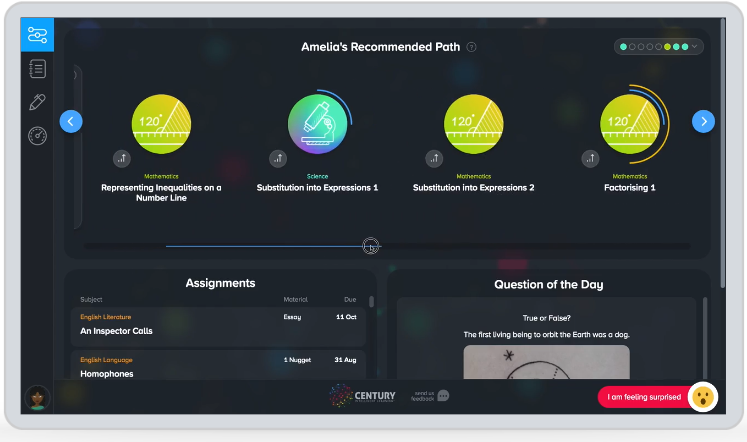
\includegraphics[width=0.7\linewidth]{obrazky/artificial-intelligence-applications-edtech-century-tech}
	\caption{}
	\label{fig:artificial-intelligence-applications-edtech-century-tech}


\subsection{QUERIUM}
\ref{khanacademy}
Querium je aplikácia obsahujúca umelú inteligenciu ktorú používa na prispôsobenie obsahu kontrolu postupu pri riešený matematických problémov. V aplikácii žiaci počítajú príklady krok po kroku a dostávajú okamžitú spätnú väzbu, toto riešení dáva učiteľom viac času zamerať sa na jednotlivých študentov. Aplikácia taktiež poskytuje spätnú väzbu na postup študentov kde sa učitelia dozvedia v ktorých krokoch a mali špeciálne študenti problém a ktoré časti učiva je potrebné špeciálne zopakovať takže učiteľ nemusí prechádzať cez celé učivo znova a môže sa zamerať len na podstatné časti čím získajú viac času na zatiaľ neprebrané učivo.

Súčasťou Queria sú aj videa o ku témam, rýchli test ktorý preverí aké vedomosti a identifikuje slabé a silné stránky aby na základe toho prispôsobil osnovy. 




\subparagraph{vysledky:}
V roku 2014 sa 11 študentov zúčastnilo testu pred a po používaný aplikácie, vyše 90 \% študentov si zlepšilo skóre v priemere o 10 bodov a až na jedného študenta aplikácia všetkým pomohla. \ref{tabulka} \ref{querium_report} 

\end{figure}

%\pgfplotsset{width=6.6cm,compat=1.7}  
%\begin{document}  
	\begin{tikzpicture}  
	
	\begin{axis}  
	[  
	ybar,  
	enlargelimits=0.00001,  
	ylabel={\#skóre},
	xlabel={\ Students},  
	symbolic x coords={1,2,3,4,5,6,7,8,9,10,11}, % these are the specification of coordinates on the x-axis.  
	xtick=data,  
	%nodes near coords, % this command is used to mention the y-axis points on the top of the particular bar.  
	nodes near coords align={vertical},  
	]  
	\addplot coordinates {(1,315) (2,310) (3,322) (4,340) (5,339) (6,335) (7,342) (8,338) (9,338) (10,345) (11,342)};
	\addplot coordinates {(1,327) (2,332) (3,337) (4,340) (5,342) (6,342) (7,347) (8,350) (9,351) (10,351) (11,352)};  
	
	\end{axis}  
	\end{tikzpicture}  

\subsection{Cognii}
\ref{cognii}
je inteligentný asistent ktorý v reálnom čase vyhodnocuje ústne odpovede študentov či eseje na základe naturel language processingu, podľa CEO Cognii si to môžeme predstaviť ako interakciu s google asistentom alebo Siri kde... my sa opýtame otázku a on odpovie. Ale v tomto prípade otázku nepoložíme my ale Cognii a my budeme odpovedať. Cognii potom odpoveď vyhodnotí a da spätnú väzbu na to čo by sme mohli zmeniť. 

Tento softvér bol nainštalovaný na Colorádsku univerzitu pre študentov filozofie. 
Spôsob krátkych odpovedí je vhodnejší z viacerých hľadísk, študent je donútený odpoveď formulovať sám z vlastných znalostí na rozdiel od napríklad testu z viacerými možnosťami kde študenti skôr vylučujú možnosti ktoré nie sú správne, táto forma  teda vyžaduje menšie množstvo vedomostí a nie tak vysoké schopnosti no z časového hľadiska je výhodnejšia.


\subsection{Khan Academy}
používa softvér ktorý vyhodnocuje úspešnosť testov na základe pravdepodobnosti s akou vyriešite ďalší problém.  Čiže na rozdiel od pôvodného hodnotenia vedomostí kde bolo sa počítalo 10 správnych odpovedí v rade, pracujú na hodnotený na základe obťažnosti otázky čo považujú za férovejší spôsob.\label{khan_academy_learning}


\subsection{ine študijne aplikacie}
Ďalšie aplikácie na pomoc študentom ako napríklad Nuance, na prepisovanie daného textu na poznámky alebo iné na prepísanie textu z fotografie na textový súbor, aplikácie ktoré budú pomáhať študentom pri zadeľovaný času na aby maximalizovali schopnosť prijímať informácie, aplikácie ktoré budú pomáhať s výslovnosťou či pri riešený matematických problémov a mnohé iné.


\section{psychologický aspekt evzdelavanie }
E-vzdelávanie má ako všetko svoje výhody aj nevýhody, môže poskytnúť študentom viac času keďže nemusia cestovať a zúčastňovať sa hodín fyzicky, vďaka čomu je možne študovať v čase v ktorom to najviac vyhovuje študentovi, ale na druhej strane tím utrpí aspekt socializácie, tento fakt je dôležitý hlavne v súčasnej dobe pandémie kde je celospoločenská socializácia značne obmedzená, ale je nutné podotknúť že za iných okolností by práve aspekt e-vzdelávania mohol pomôcť k lepšej sociálnej zrelosti žiakov preto že to je oblasť kde by sa presunula časť mimo elektronických systémov a verím že táto časť by stále prebiehala offline.


\section{Záver}
\cite{AI}Umelá inteligencia napojená pomocou vysokorýchlostného pripojenia je schopná využívať data mining algoritmus v reálnom čase a tým odokrývať nám nepoznané prepojenia a súvislosti je schopný predefinovať spôsob akým dnes vnímame vzdelávanie ktoré je založene na metódach ktoré boli vyvinuté už pred rokmi a nebrali do úvahy technologické možnosti budúcnosti. Aj preto je veľmi dôležité zamerať sa na všetky možnosti a skúsiť ich naplno využiť.

\subsection{ako e vzdelavanie ovplvnilo školstvo}
E-zdelávanie postupne už dlhšie preniká do školstva kde pôsobí pozitívny pokrok tým že poskytlo prístup k mnohým materiálom napríklad v súčasnosti je veľké množstvo videí a vyučovacích programov dostupných online čo otvorilo možnosti keď je odborný výklad vzdialený len na pár klikov. \cite{10.1145/3399971.3399984}


\bibliography{bibligraficky_subor}

\bibliographystyle{ieeetr}
%\begin{thebibliography}{9}
	
\label{khanacademy} 
\texttt{https://www.khanacademy.org/}
\\
\label{AI} 
\texttt{https://www.nttdata.com/mm/en/digital/ai/2018/september/what-is-ai}
\date{22.11.2020}
\\
\label{querium_report}
\texttt{https://querium.com/wp-content/uploads/Querium-TSI-Math-Prep-Spring-2014-Beta-Test-Preliminary-Results.pdf}

\label{cognii}
\texttt{ Xconomy: Colorado state, meet cognii: Artificial intelligence in education (2016). . Chatham: Newstex. Retrieved from https://search.proquest.com/blogs,-podcasts,-websites/xconomy-colorado-state-meet-cognii-artificial/docview/1793105199/se-2?accountid=50235}


\label{khan_academy_learning}
\texttt{http://david-hu.com/2011/11/02/how-khan-academy-is-using-machine-learning-to-assess-student-mastery.html}
	
%\end{thebibliography}

\end{document}

